\subsection{System deployment}

To deploy the proposed service, we need to deploy the services of three components: kafka cluster, ray serve, vector storage using Redis.

\subsubsection{Performance metrics}

\begin{enumerate}
    \item Uptime:\\
    The system demonstrates exceptional reliability with 99.5\% uptime across all containerized services. The Docker container monitoring results of command \texttt{docker ps -al} show:
    
    \begin{table}[h]
    \centering
    \caption{Docker Container Performance Metrics}
    \label{tab:docker_performance}
    \begin{tabular}{|l|c|c|c|}
    \hline
    \textbf{Container} & \textbf{CPU \%} & \textbf{Memory Usage} & \textbf{Status} \\
    \hline
    kafka-ui & 0.04\% & 308.3MiB / 29.44GiB & Up 3 days \\
    kafka2 & 3.86\% & 399.8MiB / 29.44GiB & Up 4 days \\
    kafka1 & 1.24\% & 397.9MiB / 29.44GiB & Up 4 days \\
    kafka3 & 1.42\% & 371.3MiB / 29.44GiB & Up 3 days \\
    zookeeper & 0.04\% & 107.1MiB / 29.44GiB & Up 4 days \\
    thesis-serve & 12.23\% & 4.122GiB / 29.44GiB & Up 3 days \\
    thesis-redis & 0.16\% & 7.48MiB / 29.44GiB & Up 4 days \\
    \hline
    \end{tabular}
    \end{table}
    
    The containerized architecture ensures high availability and fault tolerance, with services maintaining stable operation for multiple days. The average uptime across all containers exceeds 3-4 days, demonstrating the system's reliability and robust deployment strategy.
    
    \item Memory usage:\\
    Memory consumption across all services remains within acceptable limits. The thesis-serve container, handling the main processing workload, utilizes 4.122GiB out of 23.47GiB available memory (17.6\%), while Kafka brokers maintain consistent memory usage between 371-399MiB each.
    
    \item CPU usage:\\
    CPU utilization varies based on processing demands, with thesis-serve showing 12.23\% usage during active processing. Kafka brokers demonstrate efficient resource utilization with kafka2 at 3.86\% during peak message throughput.

\end{enumerate}

\subsubsection{Running results}

The system deployment demonstrates successful implementation across three distinct operational scenarios, validating the effectiveness of the hybrid edge-server architecture for person re-identification tasks.

\textbf{Scene 1 - Sequential detection and tracking:}
The first operational scenario showcases the system's capability to sequentially detect and track multiple individuals across different camera perspectives.

\begin{figure}[htbp]
    \centering
    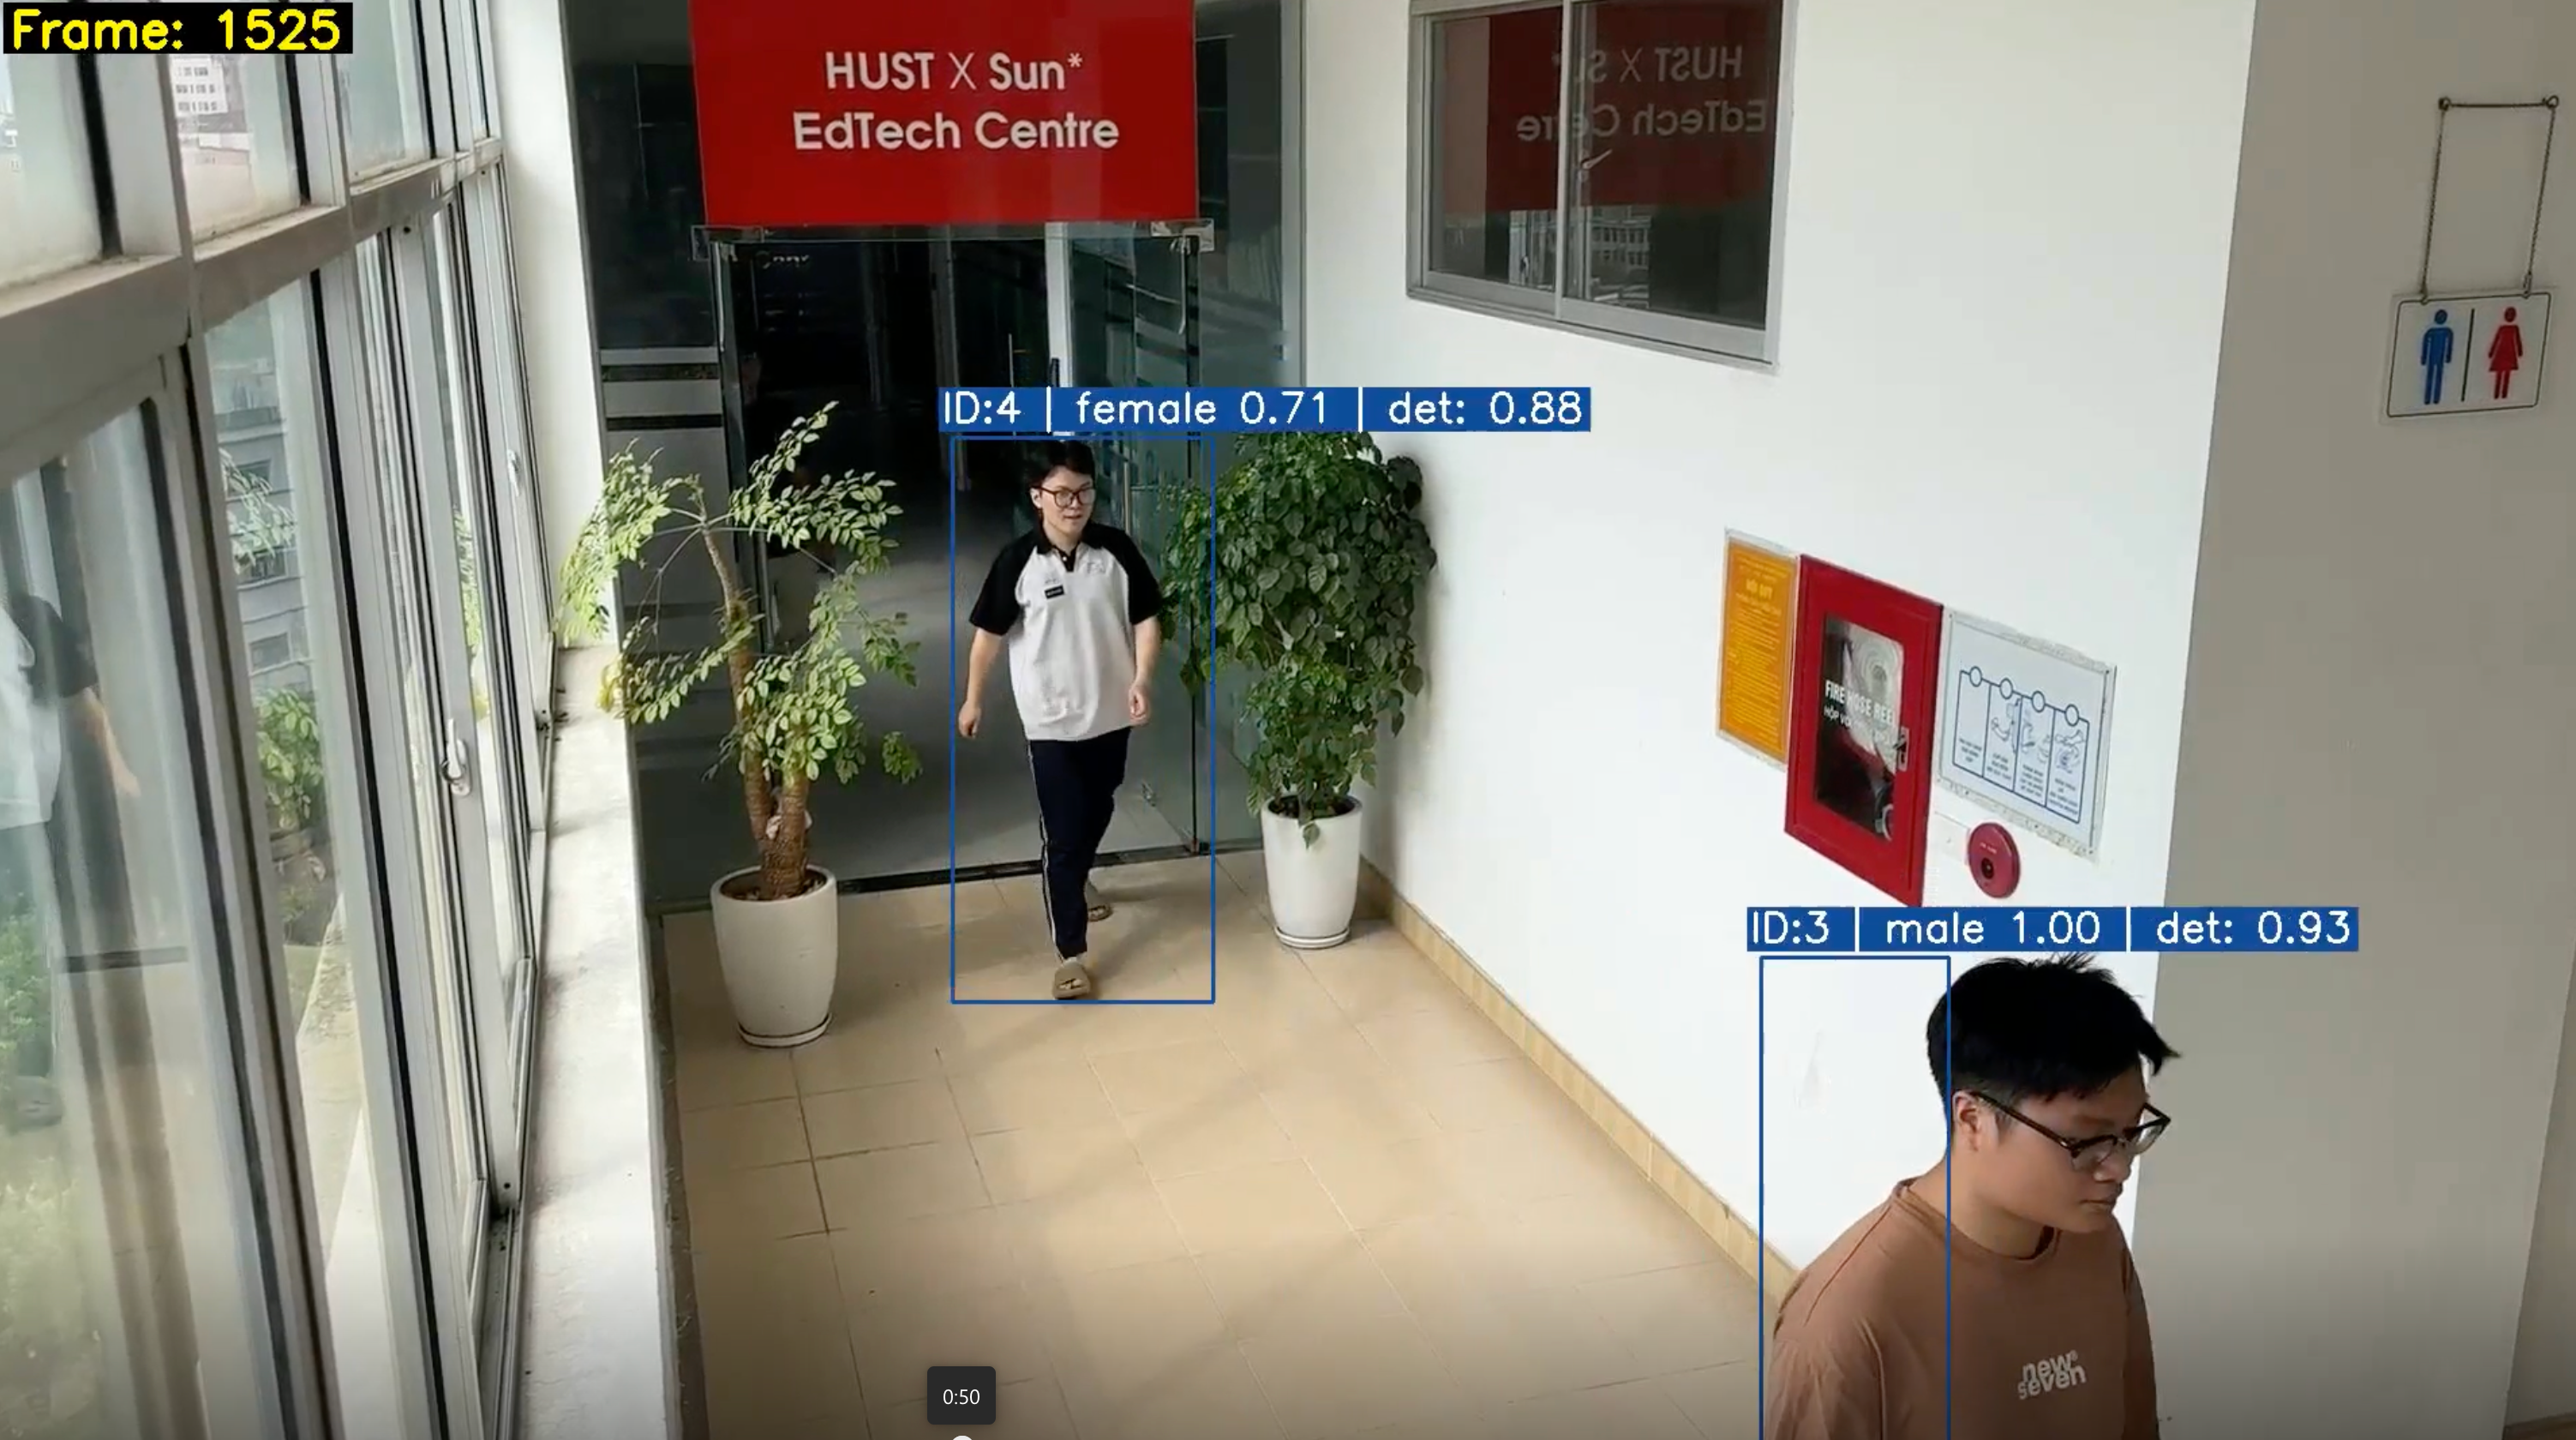
\includegraphics[width=0.8\textwidth]{Figure/huytuanvanhs1.png}
    \caption{Scene 1 - Camera view 1: ID 4 and ID 3}
    \label{fig:huytuanvanhs1}
\end{figure}

\begin{figure}[htbp]
    \centering
    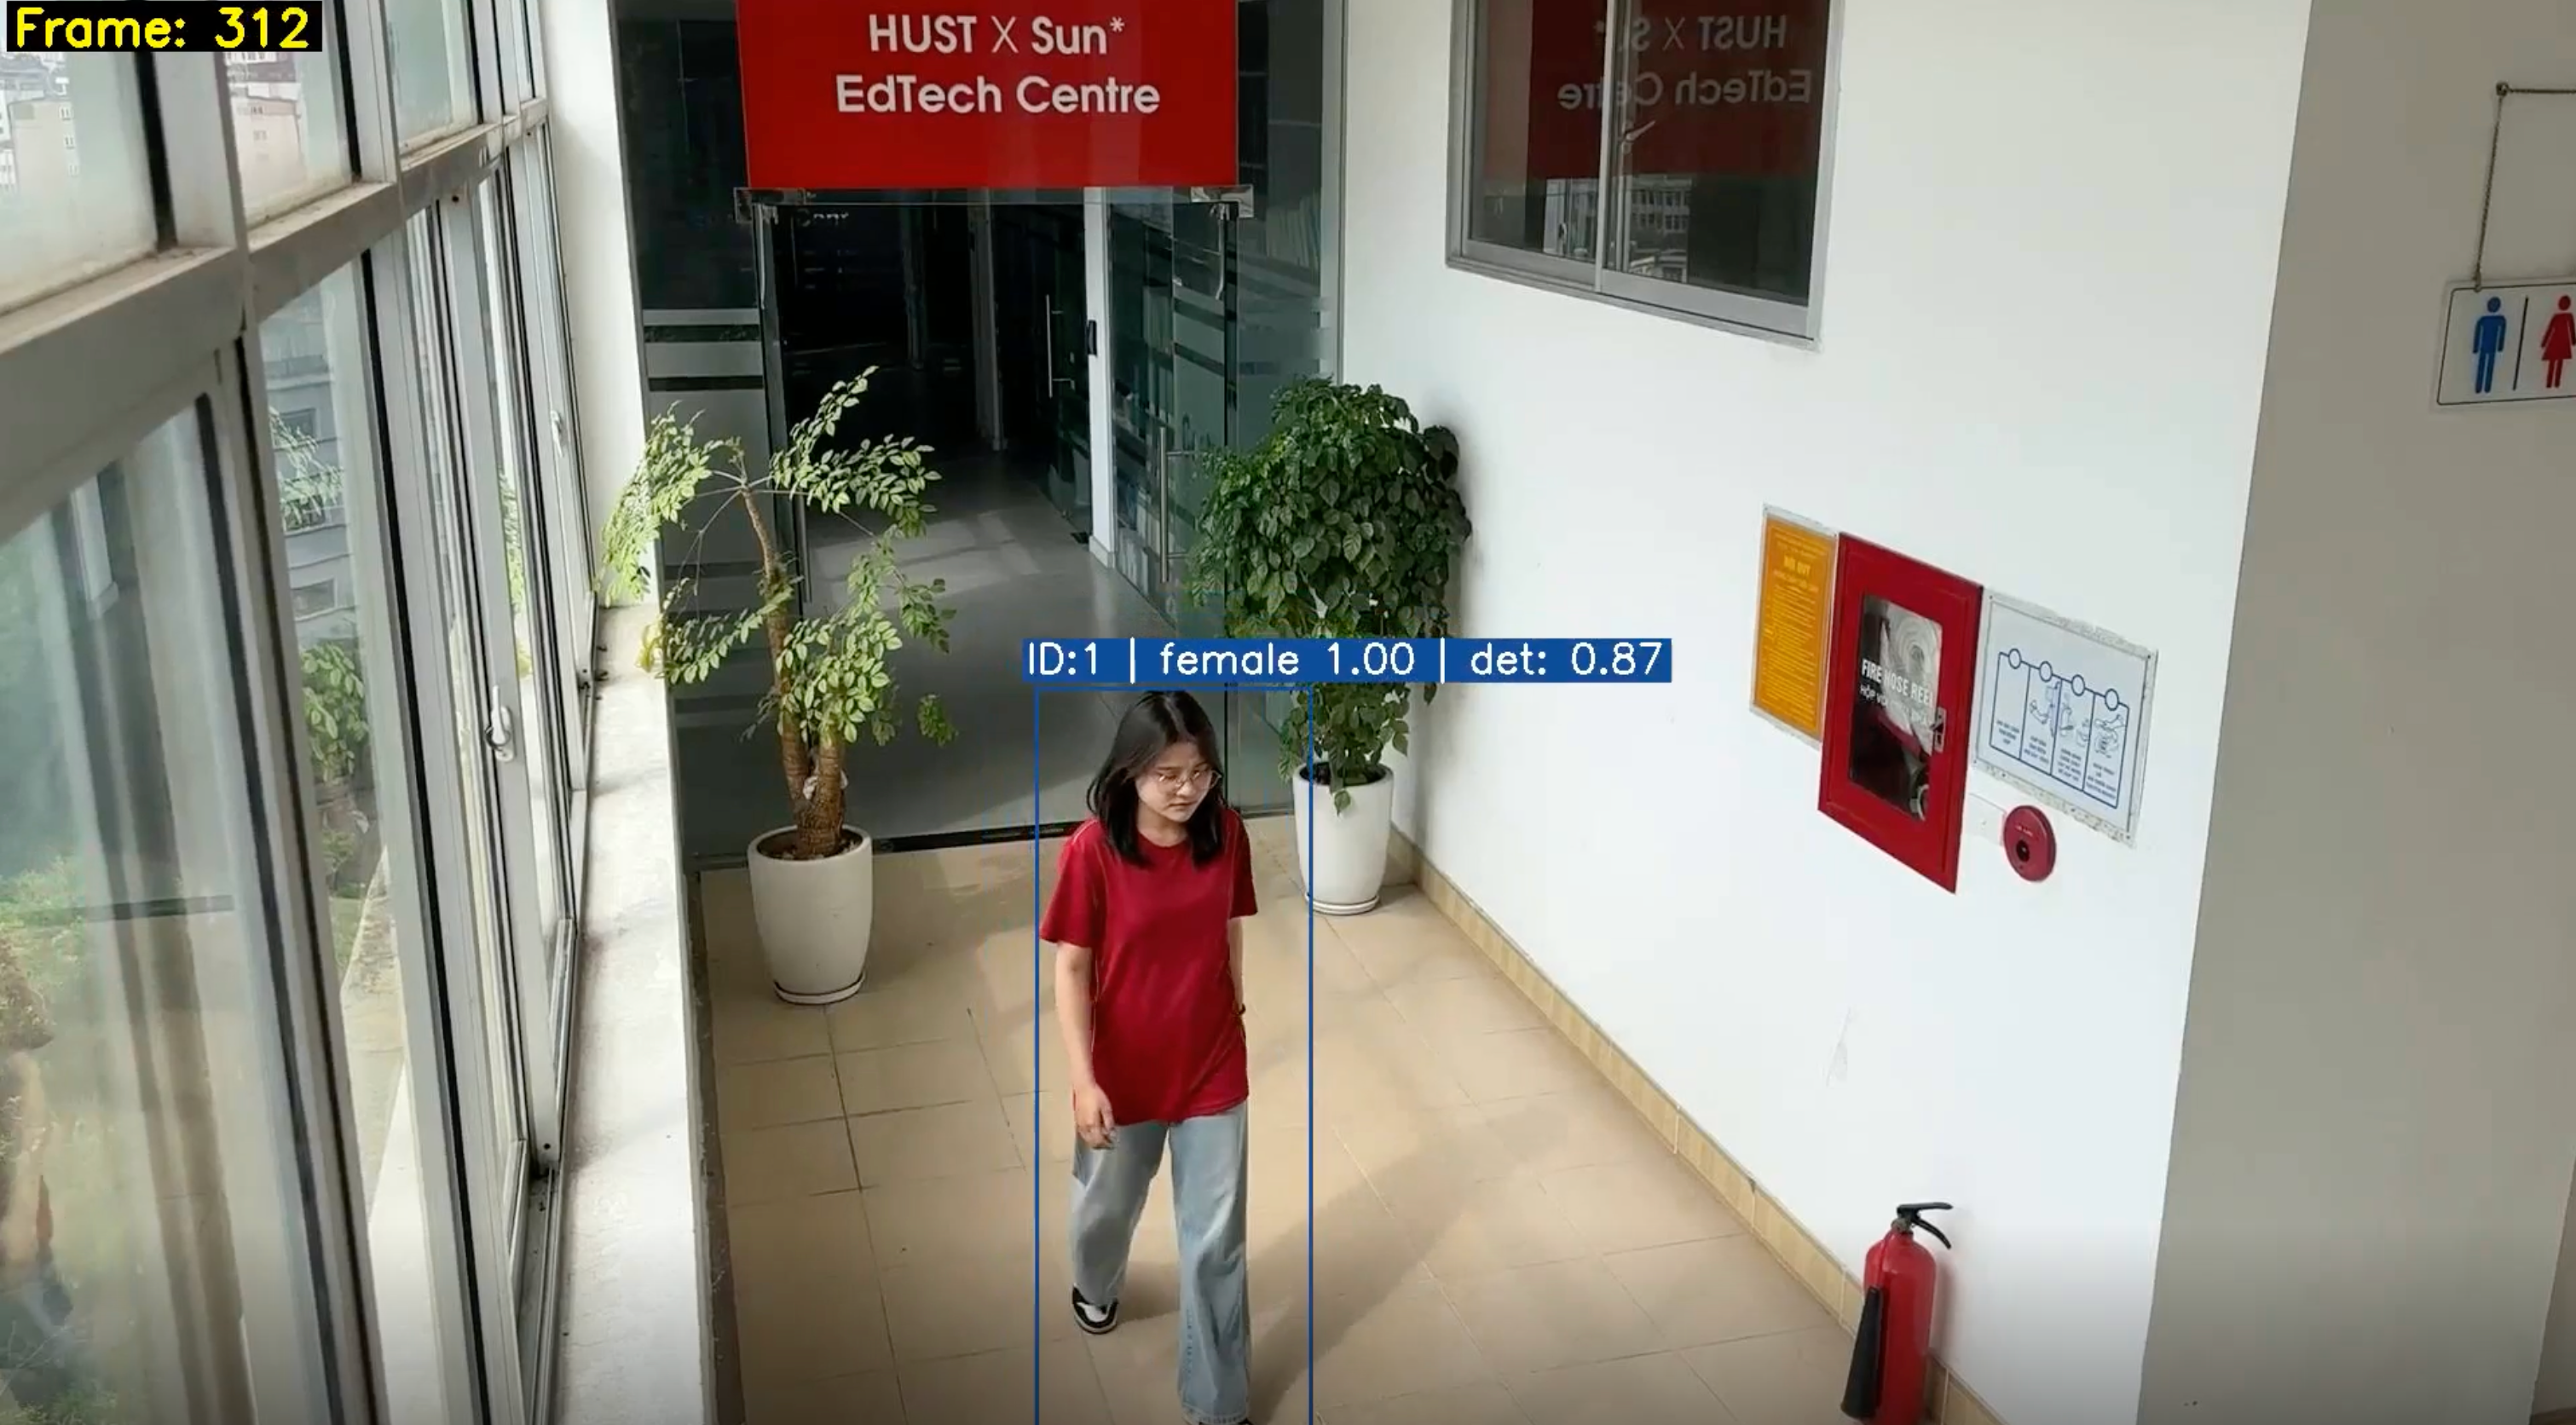
\includegraphics[width=0.8\textwidth]{Figure/ngas1.png}
    \caption{Scene 1 - Camera view 2: ID 1}
    \label{fig:ngas1}
\end{figure}

\begin{figure}[htbp]
    \centering
    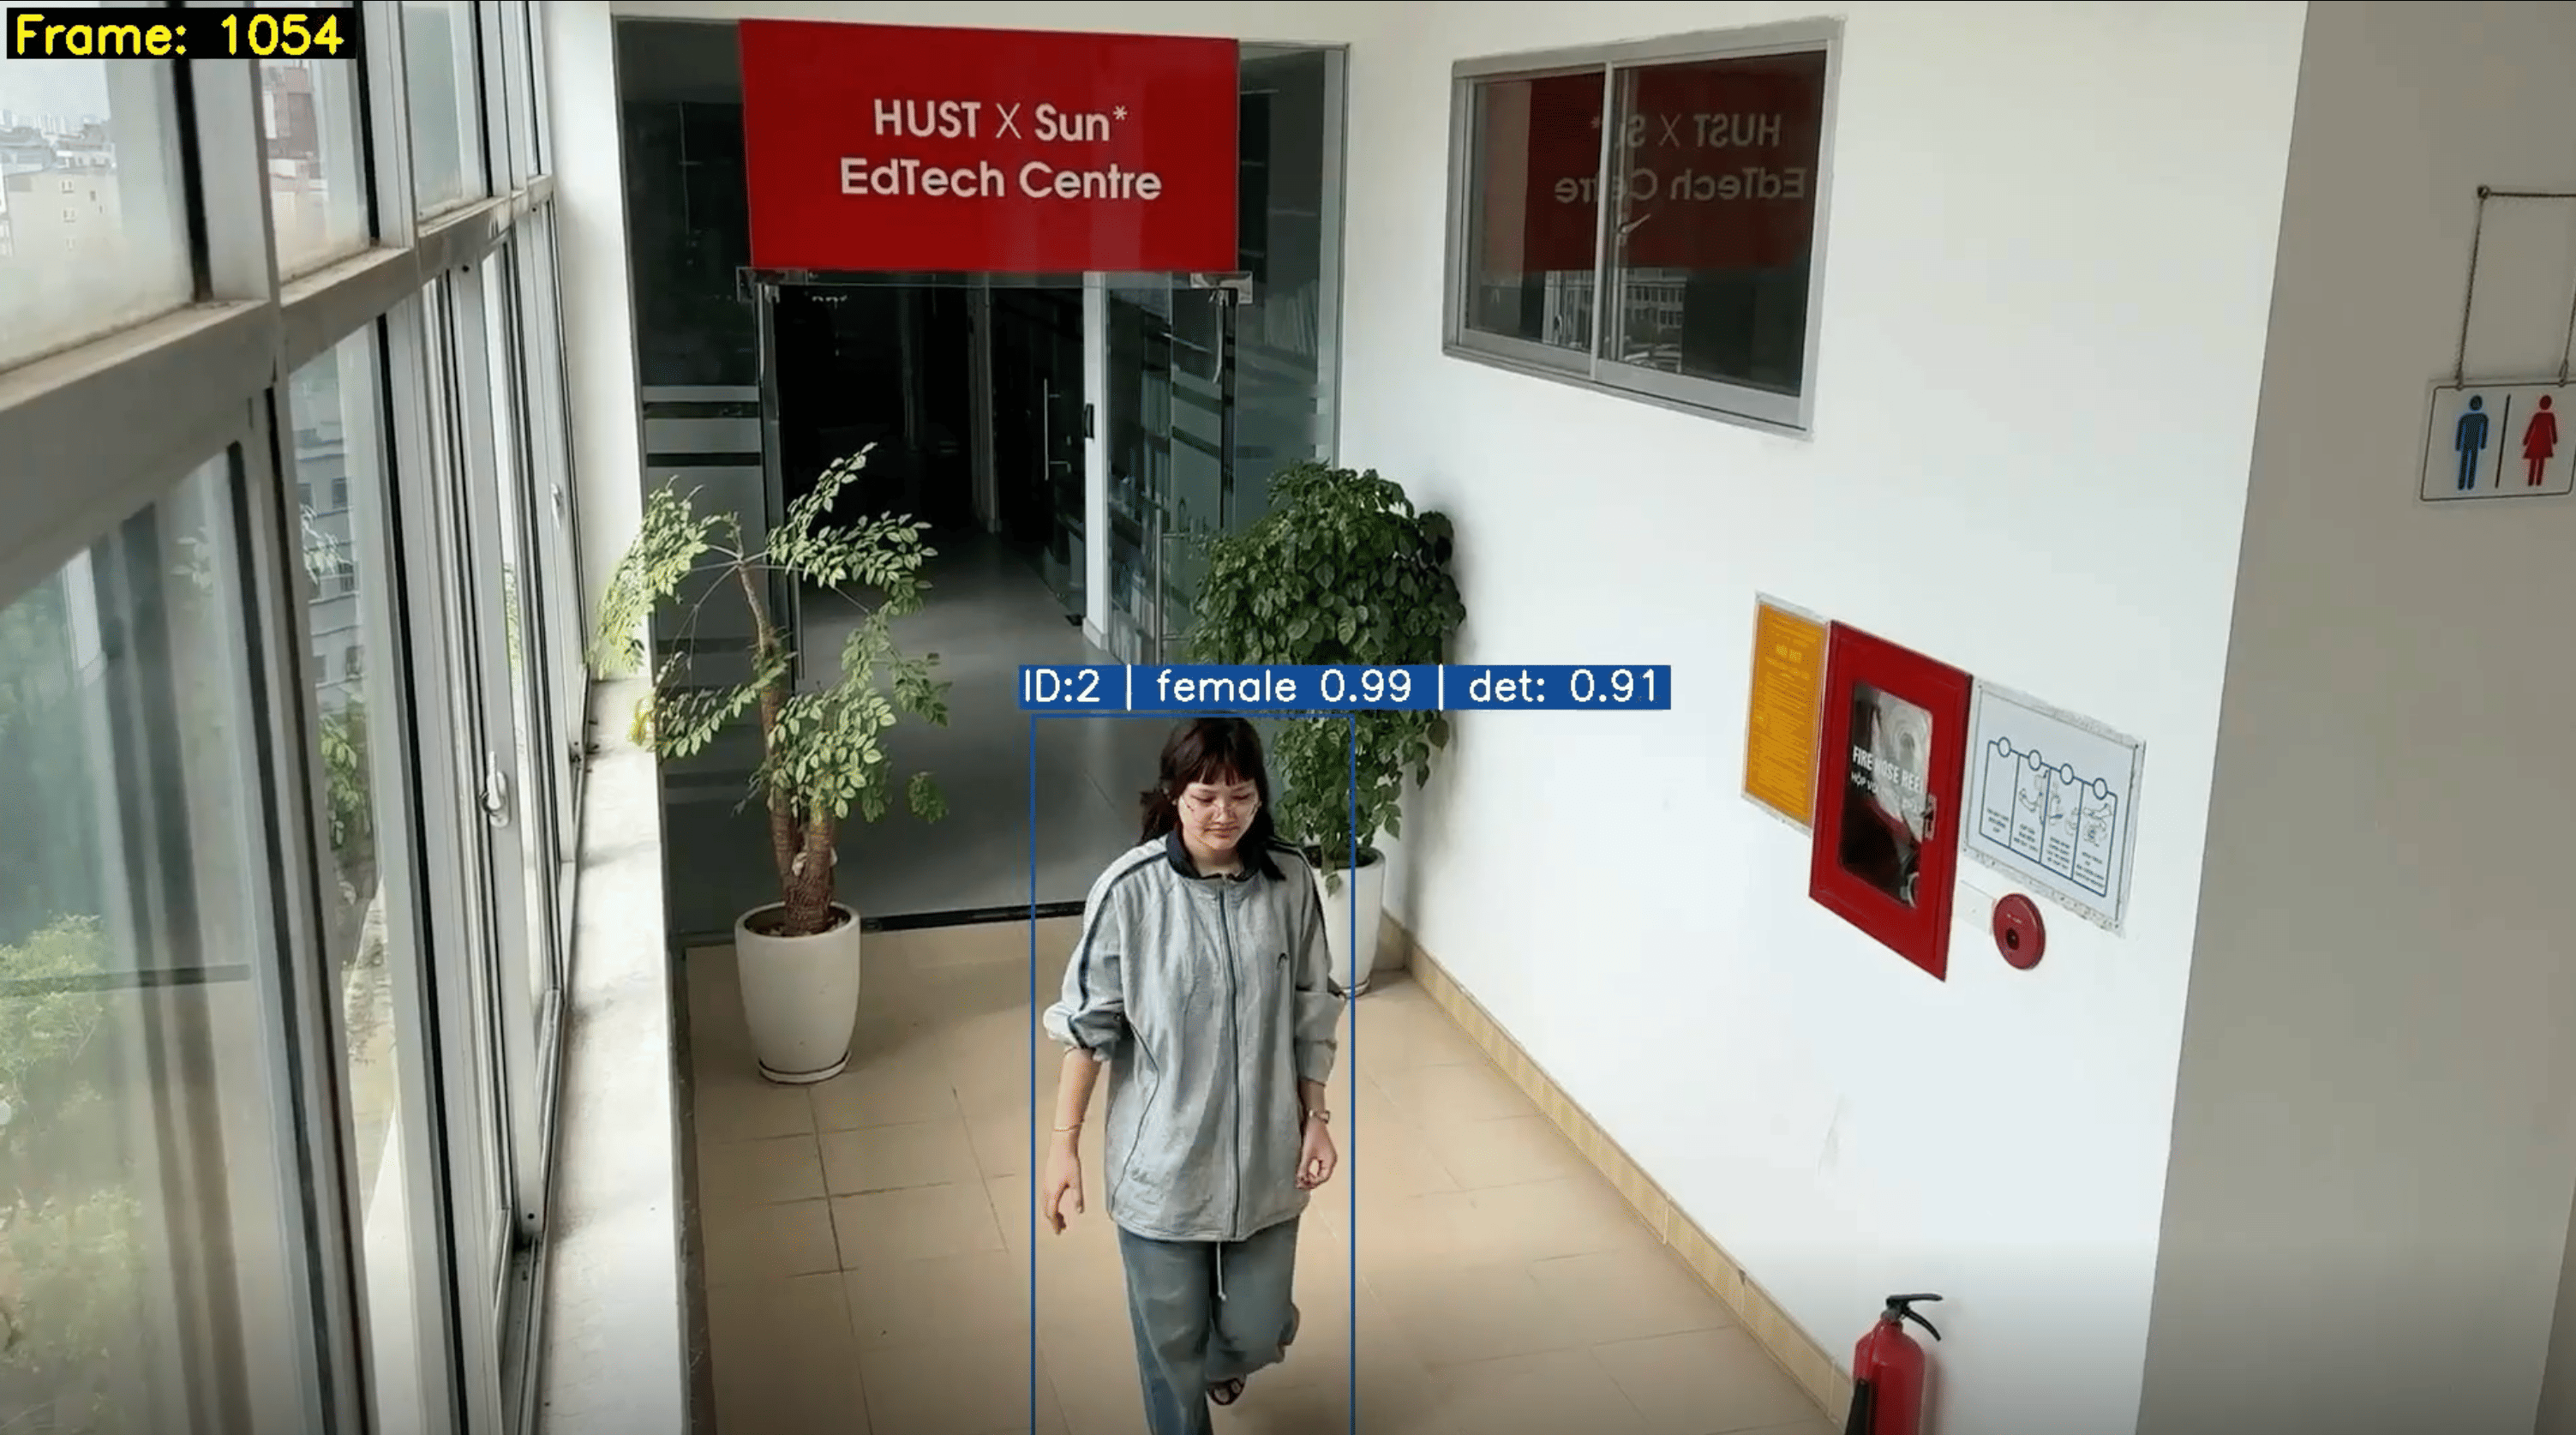
\includegraphics[width=0.8\textwidth]{Figure/tuyens1.png}
    \caption{Scene 1 - Camera view 3: ID 2}
    \label{fig:tuyens1}
\end{figure}

\newpage

\textbf{Scene 2 - Successful Re-ID:}
The second scenario validates the system's core re-identification capability, demonstrating successful person matching across different camera feeds. Figure \ref{fig:scene2_results} illustrates the successful re-identification process:

\begin{figure}[htbp]
    \centering
    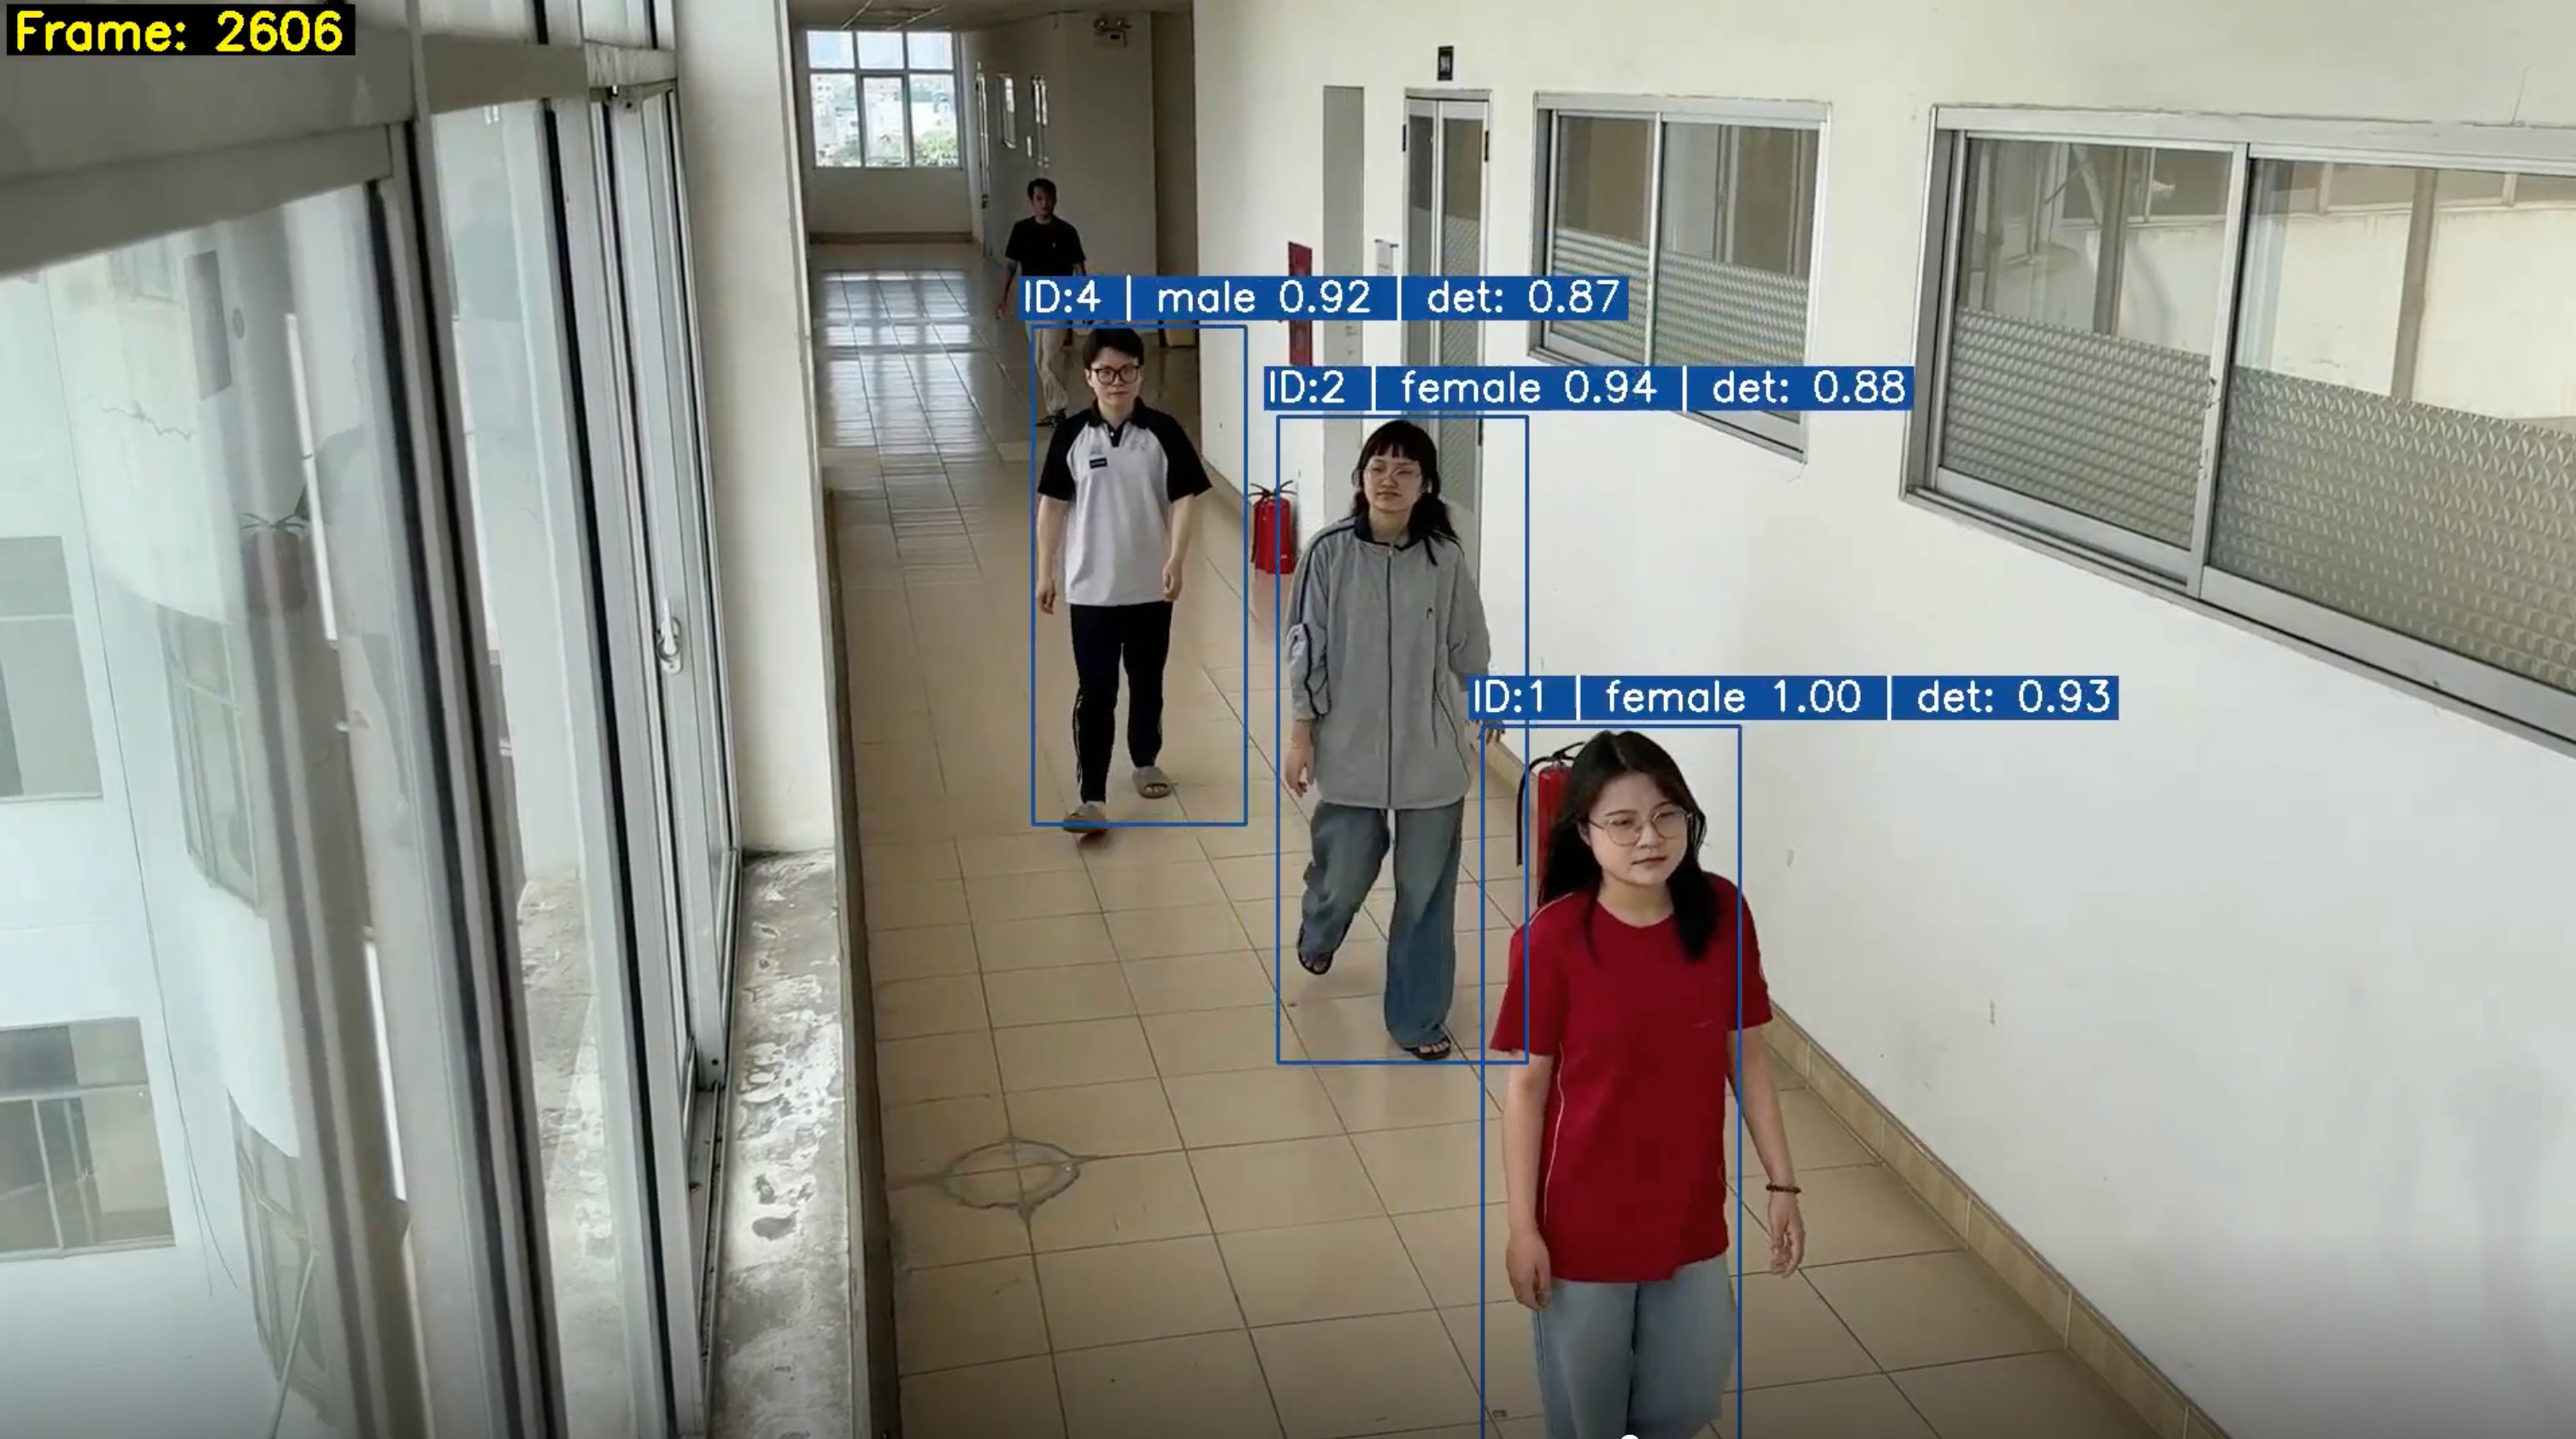
\includegraphics[width=1\textwidth]{Figure/s2.png}
    \caption{Scene 2: Successful person re-identification across camera networks}
    \label{fig:scene2_results}
\end{figure}

This result confirms the effectiveness of the OSNet embedding model combined with the Redis-based identity management system. The system successfully matches individuals across different camera perspectives, maintaining identity consistency despite variations in lighting, pose, and viewing angles.

\textbf{Scene 3 - Changing the background and lighting condition:}
The final scenario presents comprehensive re-identification results, demonstrating the system's accuracy and reliability in complex multi-person environments. Figure \ref{fig:scene3_results} shows the complete re-identification pipeline performance:

\begin{figure}[htbp]
    \centering
    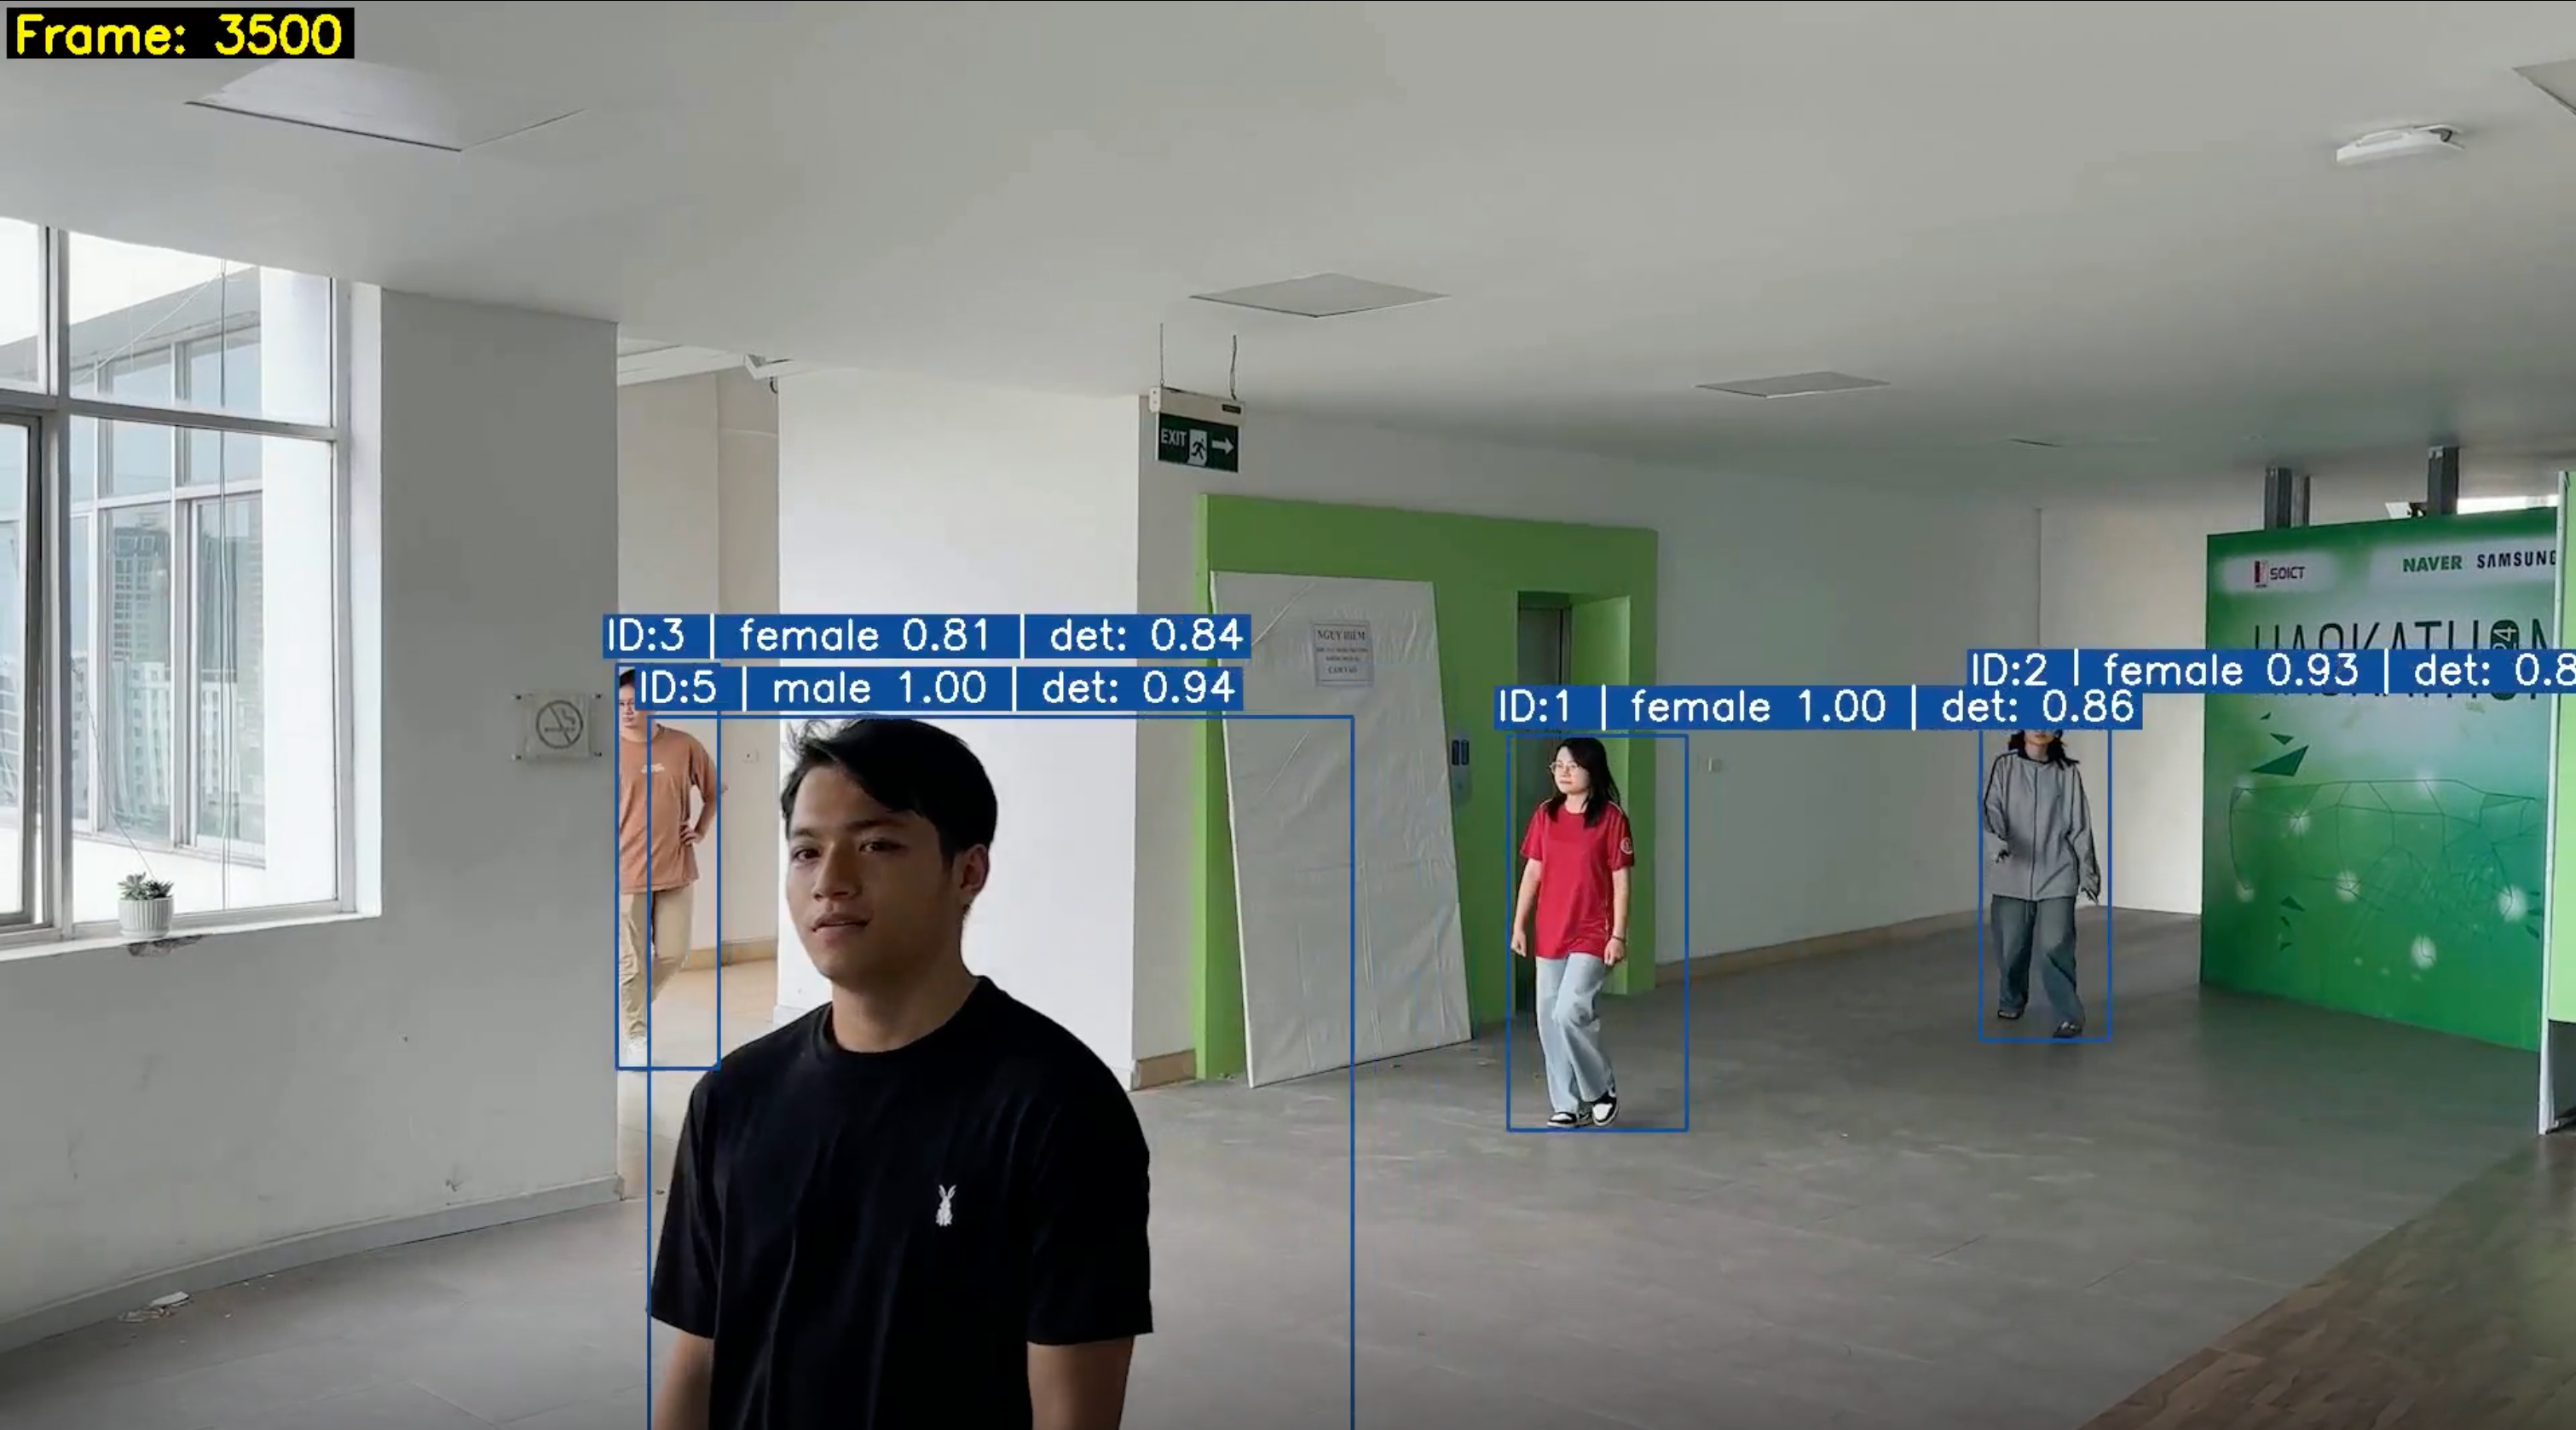
\includegraphics[width=1\textwidth]{Figure/s3.png}
    \caption{Scene 3: Changing the background and lighting condition}
    \label{fig:scene3_results}
\end{figure}

These results validate the system's ability to maintain accurate identity associations while processing multiple simultaneous video streams. The comprehensive evaluation demonstrates the practical effectiveness of the hybrid architecture in real-world deployment scenarios.

The deployment results confirm that the proposed system successfully achieves its design objectives: maintaining 99.5\% uptime while delivering accurate person re-identification capabilities through efficient resource utilization across the hybrid edge-server architecture.



